\documentclass[12pt, a4paper]{article}

% Wymagane pakiety dla XeLaTeX
\usepackage{fontspec}
\usepackage{polyglossia}
\setmainlanguage{polish}

% Ustawienia strony i formatowania
\usepackage[margin=2.5cm]{geometry}
\usepackage{hyperref}
\usepackage{booktabs}
\usepackage{tabularx}
\usepackage{xcolor}
\usepackage{listings}
\usepackage{parskip}
\usepackage{graphicx}

% Konfiguracja linków
\hypersetup{
    colorlinks=true,
    linkcolor=blue,
    filecolor=magenta,      
    urlcolor=cyan,
    pdftitle={Sprawozdanie z projektu - IoT},
}

% Konfiguracja bloków kodu
\lstset{
    basicstyle=\ttfamily\small,
    backgroundcolor=\color{gray!10},
    frame=single,
    rulecolor=\color{gray!30},
    breaklines=true,
    keywordstyle=\color{blue},
    commentstyle=\color{green!60!black},
    stringstyle=\color{orange},
    showstringspaces=false,
    extendedchars=true
}

\begin{document}

% --- STRONA TYTUŁOWA ---
\begin{center}
    {\Huge \textbf{Sprawozdanie z projektu}}\\[1cm]
    {\Large \textbf{Zaawansowany system monitorowania wnętrza czołgu — bramka Raspberry Pi}}\\[1cm]
    
\includegraphics[width=0.4\textwidth]{docs/assets/logo-pb.png}\\[0.8cm]
    \rule{\textwidth}{0.4pt}\\[0.5cm]
    \textbf{Wykonawcy:} Łukasz Kotowski, Jakub Kiryłowicz, Dawid Szczawiński, Jakub Werykowski\\[0.2cm]
    \textbf{Przedmiot:} Internet rzeczy (IoT)\\[0.2cm]
    \rule{\textwidth}{0.4pt}
\end{center}
\vspace{1cm}

% --- SEKCJONOWANIE ---
\section{Wprowadzenie}
W ramach projektu z przedmiotu \textbf{Internet rzeczy (IoT)} zaprojektowaliśmy i zaimplementowaliśmy zaawansowany system monitorowania wnętrza czołgu oparty na architekturze węzły–bramka. System składa się z co najmniej trzech węzłów pomiarowych (mikrokontrolery ESP32), bramki agregującej dane (Raspberry Pi 3) oraz warstwy wizualizacji dostępnej w sieci lokalnej.

Celem projektu było spełnienie wymagań laboratoryjnych dotyczących:
\begin{itemize}
    \item minimum \textbf{3 węzłów IoT} i \textbf{2 czujników} pomiarowych,
    \item komunikacji \textbf{MQTT} z \textbf{szyfrowaniem TLS},
    \item przechowywania historii pomiarów w bazie danych,
    \item prezentacji wyników w panelu webowym z aktualizacją na żywo.
\end{itemize}

\section{Opis systemu}
Zbudowany przez nas system realizuje następujące funkcje:

\begin{table}[htbp]
    \centering
    \renewcommand{\arraystretch}{1.3}
    \begin{tabularx}{\textwidth}{@{} >{\raggedright\arraybackslash}p{3cm} >{\raggedright\arraybackslash}p{5cm} X @{}}
        \toprule
        \textbf{Warstwa} & \textbf{Rola} & \textbf{Technologie} \\
        \midrule
        Węzły pomiarowe & Zbieranie danych z czujników, publikacja MQTT & ESP32, Arduino IDE, PubSubClient \\
        Broker MQTT & Pośrednictwo w wymianie wiadomości, szyfrowanie TLS & Mosquitto (Docker / natywnie na RPi) \\
        Bramka & Subskrypcja pomiarów, zapis do bazy, API HTTP/WS & Raspberry Pi 3, Python, FastAPI \\
        Wizualizacja & Dashboard z kartami węzłów i wykresami historii & HTML, CSS, JavaScript, Chart.js \\
        \bottomrule
    \end{tabularx}
\end{table}

Węzły ESP32 mierzą m.in. \textbf{temperaturę} (czujnik TMP102 / planowany BME680), a w rozszerzonej wersji systemu przewidziano dodatkowo pomiar \textbf{odległości} (HC-SR04) oraz \textbf{natężenia światła} (LDR). Dane są interpretowane jako parametry środowiskowe kluczowe dla bezpieczeństwa i świadomości sytuacyjnej załogi wewnątrz czołgu. Do testów i demonstracji bez sprzętu przygotowaliśmy \textbf{symulator trzech węzłów}, który publikuje dane w identycznym formacie JSON co firmware ESP32.

\begin{verbatim}
ESP32 (wezel) --MQTT/TLS :8883, JSON--> Mosquitto (broker)
Mosquitto (broker) <--HTTP/WS, mqtts--> Raspberry Pi GW
Raspberry Pi GW --> Web UI / API
Raspberry Pi GW --> SQLite DB
\end{verbatim}

\section{Architektura i struktura repozytorium}
Projekt podzieliliśmy na moduły odpowiadające poszczególnym elementom systemu:

\begin{verbatim}
iot/
├── config.yaml                  konfiguracja bramki (MQTT + TLS, baza, web)
├── docker-compose.yml           Mosquitto w kontenerze (dev)
├── docs/assets/                 materiały dokumentacyjne (logo PB)
├── mosquitto/
│   ├── config/                  mosquitto.conf, conf.d/tls.conf, passwd
│   └── certs/                   CA + certyfikat serwera (generowane skryptem)
├── esp32/weather_node/          firmware ESP32 (Arduino IDE, MQTT TLS)
├── raspberry/                   aplikacja Raspberry Pi (FastAPI + MQTT + SQLite)
└── tools/
    ├── generate_mqtt_certs.ps1  generowanie PKI (Windows)
    ├── generate_mqtt_certs.sh   generowanie PKI (Linux / RPi)
    ├── mqtt_passwd.py           generator pliku haseł Mosquitto
    └── simulator.py             symulator 3 węzłów ESP32 (MQTT TLS)
\end{verbatim}

\subsection{Węzły ESP32}
Na każdym węźle zaimplementowaliśmy:
\begin{itemize}
    \item połączenie Wi-Fi z siecią lokalną,
    \item synchronizację czasu NTP (timestamp w formacie ISO 8601),
    \item bezpieczne połączenie MQTT over TLS z weryfikacją certyfikatu CA,
    \item cykliczną publikację pomiarów co 2 sekundy na topic \texttt{weather/<node\_id>/data}.
\end{itemize}
Identyfikatory węzłów skonfigurowaliśmy zgodnie z plikiem \texttt{config.yaml}: \texttt{esp32-01} (Przedział kierowcy), \texttt{esp32-02} (Przedział bojowy), \texttt{esp32-03} (Przedział napędowy).

\subsection{Bramka Raspberry Pi}
Aplikacja bramki (Python / FastAPI) realizuje:
\begin{itemize}
    \item subskrypcję wszystkich węzłów (\texttt{weather/+/data}) z QoS 1,
    \item walidację i zapis pomiarów do bazy \textbf{SQLite},
    \item REST API do odczytu bieżących i historycznych danych,
    \item strumień WebSocket (\texttt{/ws}) do aktualizacji dashboardu w czasie rzeczywistym,
    \item panel webowy z kartami węzłów oraz wykresami temperatury, odległości i natężenia światła.
\end{itemize}

\subsection{Bezpieczeństwo komunikacji}
Zgodnie z wymaganiami projektu zabezpieczyliśmy warstwę transportową protokołu MQTT:
\begin{itemize}
    \item broker nasłuchuje na porcie \textbf{8883} (TLS),
    \item wygenerowaliśmy własną infrastrukturę PKI (CA + certyfikat serwera),
    \item włączyliśmy uwierzytelnianie użytkowników Mosquitto (osobne konta dla węzłów i bramki),
    \item ESP32 weryfikuje certyfikat CA zapisany w pamięci firmware.
\end{itemize}

\begin{table}[htbp]
    \centering
    \renewcommand{\arraystretch}{1.3}
    \begin{tabularx}{\textwidth}{@{} l X @{}}
        \toprule
        \textbf{Element} & \textbf{Wartość domyślna (dev)} \\
        \midrule
        Port TLS & \texttt{8883} \\
        Użytkownik ESP32 / symulator & \texttt{esp32\_user} \\
        Użytkownik bramki RPi & \texttt{rpi\_gateway} \\
        Hasło (dev) & \texttt{iot-dev-pass} \\
        Certyfikat CA & \texttt{mosquitto/certs/ca.crt} \\
        \bottomrule
    \end{tabularx}
\end{table}

\section{Format wiadomości MQTT}
Ustaliliśmy jednolity format payloadu JSON dla wszystkich węzłów:
\begin{itemize}
    \item \textbf{Topic:} \texttt{weather/<node\_id>/data} (np. \texttt{weather/esp32-01/data})
    \item \textbf{Payload (JSON):}
\end{itemize}

\begin{lstlisting}
{
  "node_id": "esp32-01",
  "timestamp": "2026-05-18T12:30:00Z",
  "temperature": 23.5,
  "distance": 42.0,
  "lux": 350.0
}
\end{lstlisting}

Pole \texttt{timestamp} jest opcjonalne — jeśli go nie ma, bramka stempluje pomiar czasem odbioru.\\
Pole \texttt{node\_id} w payloadzie jest opcjonalne — alternatywnie brane jest z topicu.

\section{Proces wdrożenia i uruchomienia}
Poniżej opisujemy kolejne kroki, które wykonaliśmy (lub wykonujemy) przy uruchamianiu systemu.

\subsection{Generowanie certyfikatów i haseł}
\textbf{Windows (PowerShell):}
\begin{lstlisting}
.\tools\generate_mqtt_certs.ps1
\end{lstlisting}

\textbf{Linux / Raspberry Pi 3:}
\begin{lstlisting}[language=bash]
chmod +x tools/generate_mqtt_certs.sh
./tools/generate_mqtt_certs.sh --server-cn raspberrypi.local --san-ip TWOJE_IP
\end{lstlisting}
Na produkcji ustawiamy CN/SAN na hostname lub IP Raspberry Pi (wymagane przy łączeniu po IP z ESP32).

\subsection{Uruchomienie brokera MQTT}
Wymagane pliki przed startem: \texttt{mosquitto/certs/ca.crt}, \texttt{server.crt}, \textbf{\texttt{server.key}} (generowane skryptem, nie w repozytorium).

\begin{lstlisting}[language=bash]
docker compose up -d mosquitto
\end{lstlisting}

Na Windows/macOS obraz Docker kopiuje certyfikaty i \texttt{passwd} do wewnętrznego systemu plików kontenera z poprawnymi uprawnieniami (bind mounty nie obsługują \texttt{chmod}/\texttt{chown}). Broker nasłuchuje na \textbf{8883} (TLS + hasło) oraz \textbf{1883} (plain, tylko localhost w kontenerze).

\subsection{Uruchomienie bramki Raspberry Pi}
Domyślna konfiguracja w \texttt{config.yaml} używa TLS:

\begin{lstlisting}
mqtt:
  host: "localhost"
  port: 8883
  username: "rpi_gateway"
  password: "iot-dev-pass"
  tls:
    enabled: true
    ca_file: "mosquitto/certs/ca.crt"
\end{lstlisting}

\begin{lstlisting}[language=bash]
pip install -r requirements.txt
python -m raspberry.main
\end{lstlisting}

Panel webowy jest dostępny pod adresem \texttt{http://<IP\_RPi>:8000}.

\subsection{Symulator węzłów (testy bez ESP32)}
Do weryfikacji całego łańcucha bez fizycznych mikrokontrolerów używamy symulatora:

\begin{lstlisting}[language=bash]
python tools/simulator.py --host localhost --port 8883 --interval 2
\end{lstlisting}
Symulator emuluje trzy węzły z lekko różniącymi się profilami pomiarowymi (temperatura, odległość, lux).

\subsection{Wgranie firmware na ESP32}
\begin{enumerate}
    \item Otwieramy \texttt{esp32/weather\_node/WeatherNode.ino} w Arduino IDE.
    \item Instalujemy bibliotekę \textbf{PubSubClient} ($\ge$ 2.8) oraz \textbf{ArduinoJson}.
    \item Kopiujemy \texttt{secrets.h.example} $\rightarrow$ \texttt{secrets.h} (lub edytujemy \texttt{secure.h}).
    \item Wklejamy zawartość \texttt{mosquitto/certs/ca.crt} do \texttt{CA\_CERT}.
    \item Ustawiamy \texttt{MQTT\_HOST} na IP Raspberry Pi oraz \texttt{NODE\_ID} (np. \texttt{esp32-01}).
    \item Wgrywamy firmware — w Serial Monitorze (115200) powinno pojawić się potwierdzenie połączenia z brokerem (TLS).
\end{enumerate}

\subsection{Wdrożenie natywne na Raspberry Pi 3}
Na docelowym urządzeniu zainstalowaliśmy Mosquitto bezpośrednio w systemie:

\begin{lstlisting}[language=bash]
sudo apt install -y mosquitto mosquitto-clients openssl
./tools/generate_mqtt_certs.sh --server-cn raspberrypi.local \
  --san-ip $(hostname -I | awk '{print $1}')
sudo cp mosquitto/certs/{ca.crt,server.crt,server.key} /etc/mosquitto/certs/
sudo cp mosquitto/config/passwd /etc/mosquitto/passwd
sudo cp mosquitto/config/rpi-tls.conf.example /etc/mosquitto/conf.d/tls.conf
sudo chown mosquitto: /etc/mosquitto/certs/* /etc/mosquitto/passwd
sudo systemctl restart mosquitto
\end{lstlisting}

Test subskrypcji:
\begin{lstlisting}[language=bash]
mosquitto_sub -h localhost -p 8883 \
  --cafile mosquitto/certs/ca.crt \
  -u esp32_user -P iot-dev-pass \
  -t "weather/+/data" -v
\end{lstlisting}

\section{API HTTP bramki}
Zaimplementowaliśmy następujące endpointy:

\begin{table}[htbp]
    \centering
    \renewcommand{\arraystretch}{1.3}
    \begin{tabularx}{\textwidth}{@{} l l X @{}}
        \toprule
        \textbf{Metoda} & \textbf{Endpoint} & \textbf{Opis} \\
        \midrule
        GET & \texttt{/} & Dashboard webowy \\
        GET & \texttt{/api/health} & Status bramki + MQTT (\texttt{mqtt\_tls}, \texttt{mqtt\_port}) \\
        GET & \texttt{/api/nodes} & Lista węzłów + ostatni pomiar \\
        GET & \texttt{/api/measurements/latest} & Najnowszy pomiar dla każdego węzła \\
        GET & \texttt{/api/measurements/history?node\_id=…\&limit=…} & Historia pomiarów \\
        WS & \texttt{/ws} & Strumień pomiarów na żywo \\
        \bottomrule
    \end{tabularx}
\end{table}

\section{Wymagania środowiskowe}
\begin{itemize}
    \item Python 3.10+
    \item OpenSSL (generowanie certyfikatów)
    \item Broker Mosquitto (Docker lub natywnie na RPi)
    \item (opcjonalnie) Docker Compose
    \item Arduino IDE + biblioteki ESP32 (dla węzłów fizycznych)
\end{itemize}

\section{Wyniki i wnioski}
W ramach projektu udało nam się zrealizować kompletny łańcuch IoT: od węzłów pomiarowych, przez zabezpieczony broker MQTT, po bramkę z bazą danych i interfejsem użytkownika. System spełnia wymagania dotyczące liczby węzłów, szyfrowanej komunikacji oraz wizualizacji danych dla zaawansowanego monitorowania wnętrza czołgu w sieci lokalnej.

\textbf{Osiągnięte cele:}
\begin{itemize}
    \item działająca komunikacja MQTT over TLS między węzłami a bramką,
    \item zapis i odczyt historii pomiarów w SQLite,
    \item dashboard webowy z aktualizacją WebSocket i wykresami,
    \item symulator umożliwiający testy bez sprzętu,
    \item skrypty automatyzujące generowanie certyfikatów i haseł.
\end{itemize}

\textbf{Możliwe kierunki rozwoju:}
\begin{itemize}
    \item podłączenie czujnika \textbf{BME680} (temperatura, wilgotność, ciśnienie) oraz \textbf{HC-SR04} w firmware ESP32,
    \item rotacja certyfikatów (plik CA w SPIFFS lub NVS na ESP32),
    \item mTLS (certyfikat klienta na ESP32) dla wyższego poziomu bezpieczeństwa,
    \item alerty przy przekroczeniu progów (np. pin ALERT na TMP102).
\end{itemize}

\clearpage
\section{Dokumentacja fotograficzna}
\begin{figure}[htbp]
    \centering
    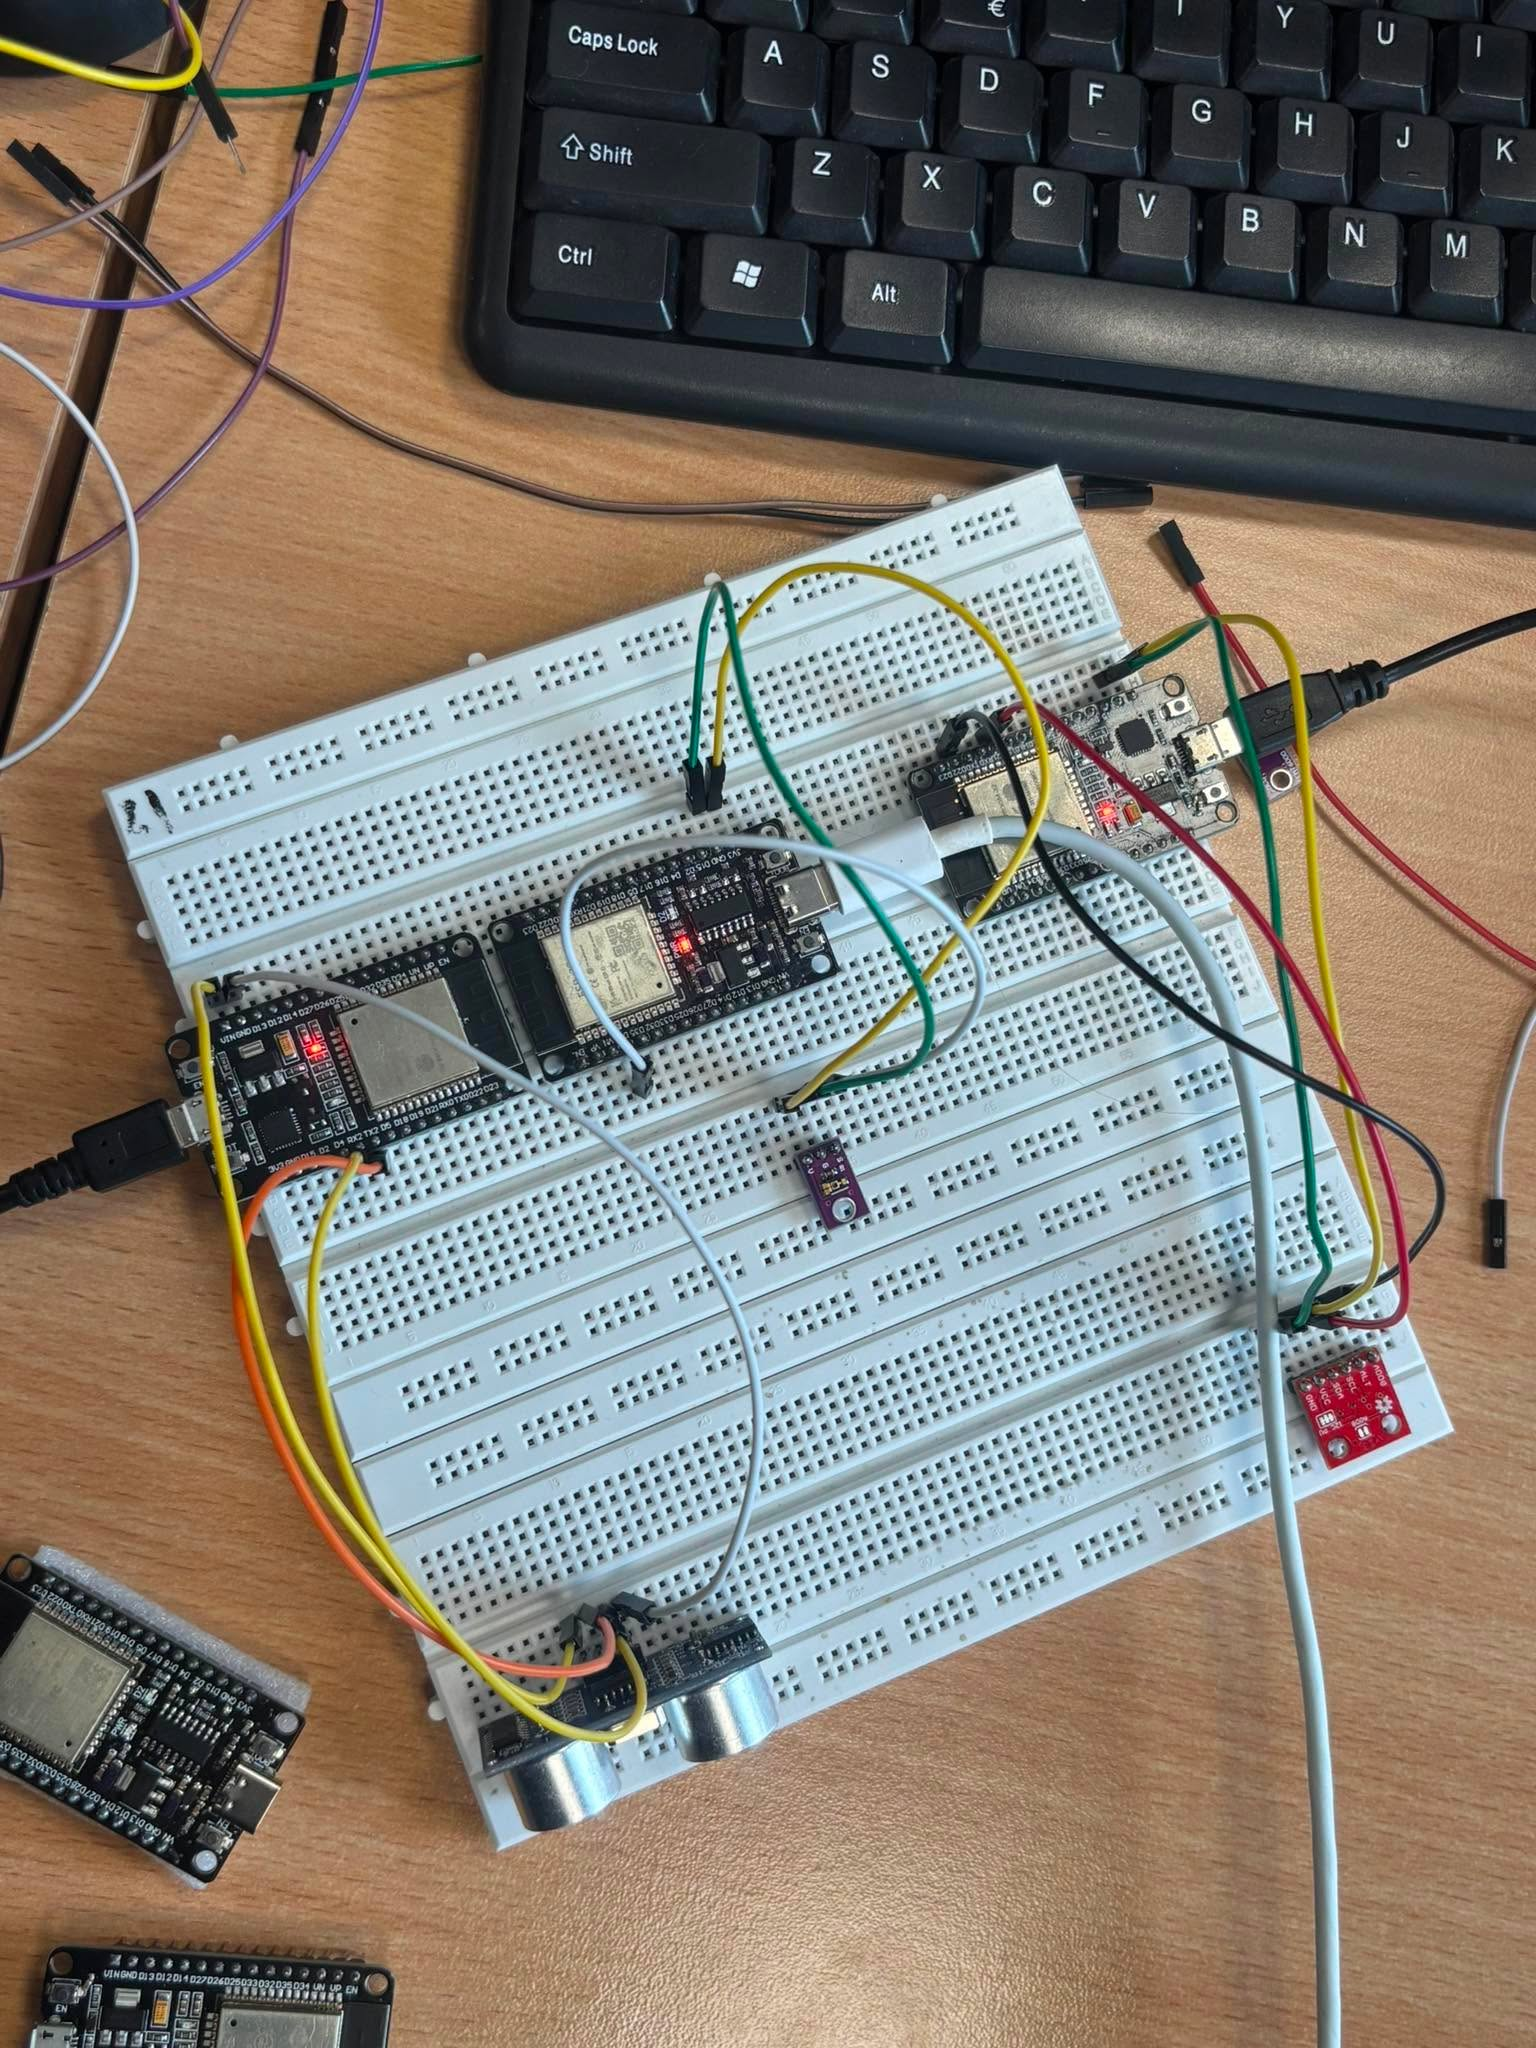
\includegraphics[width=0.8\textwidth]{fotka.jpg}
    \caption{Fotografia stanowiska projektowego}
\end{figure}

\end{document}